\section{Introduction to Microservice  Architectures}
\label{sec:techKnowHow}
This section aims to broadly elaborate the nature of microservices. First, the term will be defined and distinguished between \acrfull{soa}. After having understood that crucial part, the theory and the benefits of self-contained systems are introduced. This chapter will be finished by having a look at event-based microservice collaboration. Its advantages and disadvantages will be shown within the section. 

\subsection{Distinction Between SOA and Microservice Architectures}
Microservice architecture is a commonly used buzzword for a modern way of implementing software. Looking into data from Google Trends, it is possible to see that the popularity of this approach has been increasing dramatically since 2014. \cite{microservices}\newline
\\
A monolithic application which grew over time often leads to poor maintainability and high complexity. To avoid this, the architecture needs to be de-serialised into multiple services, which results in a service oriented architecture (SOA). But due to recent development it seems that SOA will be replaced by microservice architectures more often.\cite{mircorVSsoa}\newline
Both of those methodologies suggest the decomposition of software. Therefore, SOA focuses on integrating those services for the entire company within a centralised management and governance. Microservices instead, focus on decomposing services without global governance. This results in higher autonomy and decoupling. \cite{mircorVSsoa} A communication over REST via HTTPS, RPC or CORBA is chosen quite often.\newline
Furthermore, the coupling between the different services is considered to be low. This allows multiple development teams to work on distinct components without affecting each other. Overall it is possible to see that those teams are enabled to build and adapt components faster than with monolithic solutions. Additionally,  modern IT environments often use DevOps which can embrace their full potential of constant integration and delivery (\acrshort{ci/cd}) within a microservice  world. \cite{redHatMicroservices}\newline
\\
Next to the benefits, there are also challenges to face while moving to a decomposed architecture. Brian Atkisson, a Senior Principal Systems Engineer at Red Hat, introduces eight of them. 
\begin{itemize}
    \item Building - What versions of services are compatible to each other? Where are hidden dependencies?
    \item Testing - Integration testing is crucial and based on the dependencies. 
    \item Versioning - Each service has its own version as well as a collection of versions. The management of these collections gains complexity rapidly.
    \item Deploying - Strong automation is often necessary in order to be able to fulfil CI/CD requirements.
    \item Logging - Without centralised logging, it is extremely hard to figure out what is going on.
    \item Monitoring - Handling of service data and distributed request tracing within a centralised dashboard.
    \item Debugging - It is hard to determine within which microservice  a problem is located without proper monitoring. Even good monitoring and logging is used more often than debugging.
    \item Connectivity - The services need to be connected to each other without any hard-coded information. This topic will be discussed when having a look at the event-based and process-driven approach. 
\end{itemize}
\cite{ChallengesMicroservices}

\subsection{The Point of behind Self-Contained-Systems}
Talking about \acrfull{scs} is always about the question of how to structure and slice the microservices mentioned above.\newline
The most important characteristics is that they are licensed under a creative commons licence from the company innoQ. In total, there are eight characteristics which need to be full-filled by such an application. First of all, the SCS need to be autonomous. Due to this, all data, business logic and \acrshort{ui} needs to be contained within the application. Furthermore, the communication between multiple systems should be asynchronous and the shared infrastructure needs to be minimised. \cite{scs}\newline
\\
Eberhard Wolff gives a good outlook on the adoption of this fundamental idea on real systems. Therefore, he elaborates on how to integrate multiple SCS, targets the topic of data replication and heads forward to a possible partitioning of a costumer journey into various SCS:\newline
\begin{itemize}
    \item Integration: Since all SCS are part of a larger system, they need some way to communicate. Wolff states that the preferred way of integration is done within the UI layer. Alternatively, asynchronous communication on the business-logic layer is recommended.
    \item While talking about data replication, it is important to have a single source of truth for each piece of data. Replication is necessary in order to be able to communicate asynchronously.
    \item In order to cut a system into several SCS, Wolff proposes to use vertical decomposition. ''The systems have to be separated into multiple parts that each have a UI, logic and database''\cite{scsWolf}. By applying this idea to the customer journey, it can result in an architecture as shown in figure \ref{fig:scsJourney}.
\end{itemize}
\cite{scsWolf}\newline
\begin{figure}[!htb]
    \centering
    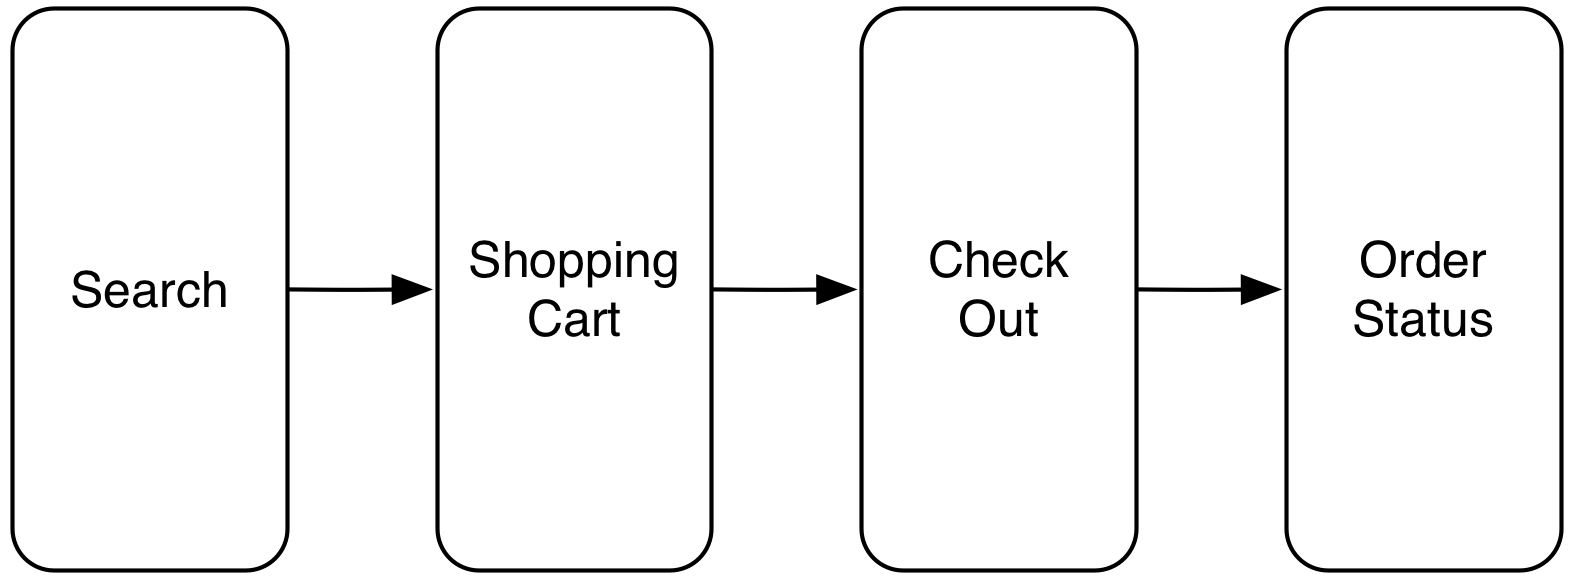
\includegraphics[scale=0.2]{pictures/Journey.png}
    \caption{Customer journey for an e-commerce system partitioned in various SCS \cite{scsWolf}}
    \label{fig:scsJourney}
\end{figure}

These fundamentals of microservices and self-contained systems are important and will be mapped on data warehouse architectures in chapter \ref{sec:finalArchitecture}.

\subsection{Integrating an Event-Based Bus into the Microservice  Landscape}
\label{sec:eventBasedArchitecture}
Making use of an event-driven choreographed architecture is opposite to using a centralised orchestrator and therefore provides loose coupling. The ''EventBus allows publish-subscribe-style communication between components without requiring the components to explicitly register with one another (and thus be aware of each other).'' \cite{EventBusExplained} \newline
Another well-known product which is often used in this context is Apache Kafka. It calls itself as ''distributed streaming platform'' having three key capabilities: First of all, publishing and subscribing to streams, storing streams as well as processing streams.\cite{kafka}
Next up, we are using this technology as an example in order to elaborate on the challenges of this approach.\newline
\\
Bernd Rücker, the Chief Technologist of Camunda, points those out with an example. Therefore, let's start by having a look at the challenges:
\begin{itemize}
    \item How to change the flow of events?
    \item How to avoid losing sight of the flow?
    \item How to manage \acrshort{sla}s and resilience of the overall flow?
    \item How to avoid wired coupling?
\end{itemize}
\cite{eventDrivenMicroservices}\newline
\\
The illustration in figure \ref{fig:chalengesChoreographedMicroservices} shows how easily a loosely coupled choreographed system can result into dependencies. Bernd Rücker chooses the common customer on-boarding process to visualise it. The first illustration in figure \ref{fig:chalengesChoreographedMicroservices} shows the services and their flow of events. Furthermore, he points out that by only adding one additional service to the overall system, such as a criminal check, an adaption of at least two other services will follow. This is shown in the second and alternatively third illustrations. \cite{eventDrivenMicroservices}\newline
\begin{figure}[!htb]
    \centering
    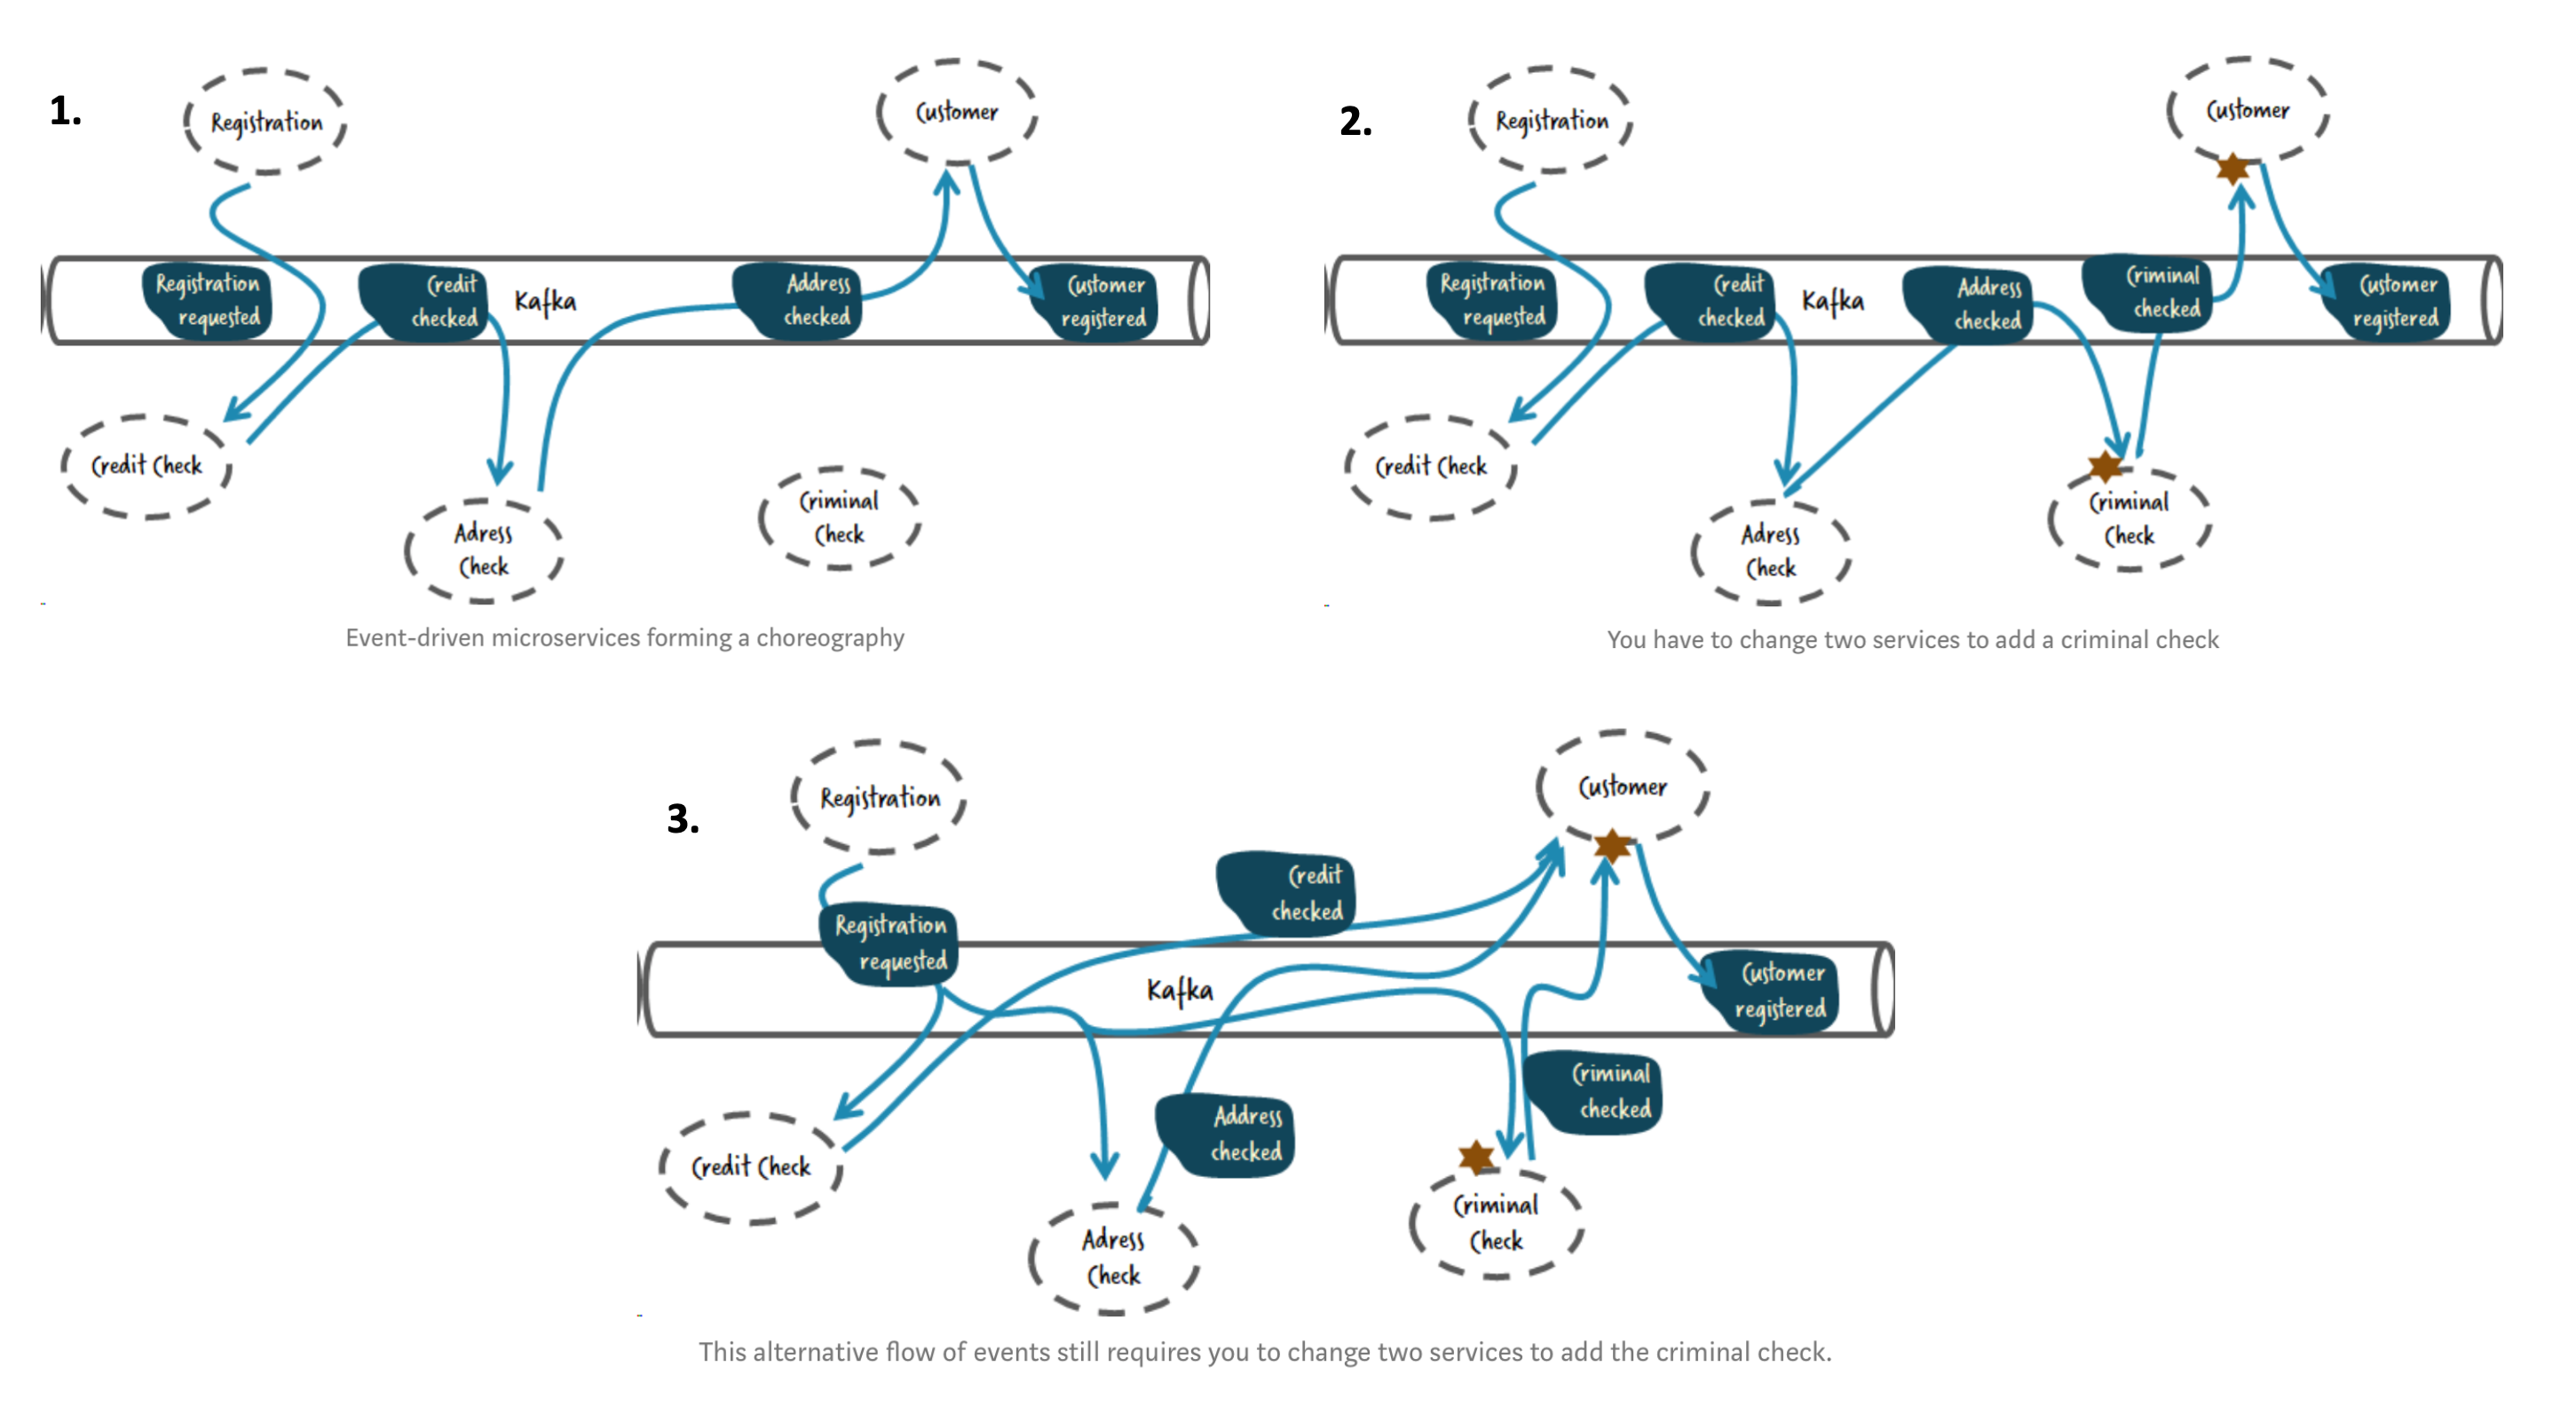
\includegraphics[scale=0.33]{pictures/FlowOfEvents.png}
    \caption{Challenges of choreographed microservices \cite{eventDrivenMicroservices}}
    \label{fig:chalengesChoreographedMicroservices}
\end{figure}\\
Summarised, this problem combined with the ''emerging behaviour that will only be experienced during runtime'' \cite{eventDrivenMicroservices} often leads to losing sight of flow.\newline
Furthermore, these faults can be seen as the transition into the next chapter where the process driven architecture will be discussed. Nevertheless, the similarities between microservices and self-contained systems with regard to data warehouse systems can be pointed out quite well. The components which are known from the reference architecture in chapter \ref{sec:referenceArchitecture} figure \ref{fig:referenceArchitecture} can be sliced along the data warehousing process into distinct SCS.\newline
The next section will now focus on how to orchestrate these properly without the challenges of an event-driven architecture. 